\chapter{Берік байланыстылық}

\index{берік байланысты граф}

Бағытталған графта қырлармен тек бір бағытта жүруге болады.
Сондықтан граф байланысты болса да, кез келген екі төбе арасында
жол болатынына кепілдік бермейді. Сондықтан байланыстықты талап етіп қана қоймайтын жаңа тұжырымдаманы анықтағанымыз жөн.

% In a directed graph,
% the edges can be traversed in one direction only,
% so even if the graph is connected,
% this does not guarantee that there would be
% a path from a node to another node.
% For this reason, it is meaningful to define a new concept
% that requires more than connectivity.

Егер әр төбеден графтағы басқа барлық
төбелерге баратын жол болса, граф берік
байланысты болады. Мысалы, төмендегі суреттің сол жағындағы граф --
берік байланысты, ал оң жағындағы граф -- берік байланысты емес.
% A graph is \key{strongly connected}
% if there is a path from any node to all
% other nodes in the graph.
% For example, in the following picture,
% the left graph is strongly connected
% while the right graph is not.

\begin{center}
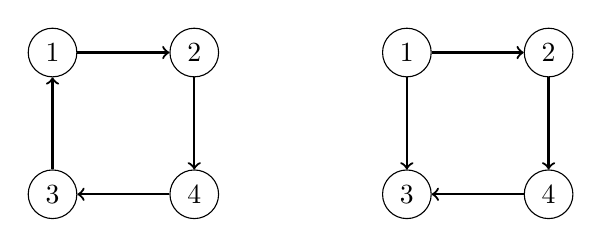
\begin{tikzpicture}[scale=0.9]
\node[draw, circle] (1) at (1,1) {$1$};
\node[draw, circle] (2) at (3,1) {$2$};
\node[draw, circle] (3) at (1,-1) {$3$};
\node[draw, circle] (4) at (3,-1) {$4$};

\path[draw,thick,->] (1) -- (2);
\path[draw,thick,->] (2) -- (4);
\path[draw,thick,->] (4) -- (3);
\path[draw,thick,->] (3) -- (1);

\node[draw, circle] (1b) at (6,1) {$1$};
\node[draw, circle] (2b) at (8,1) {$2$};
\node[draw, circle] (3b) at (6,-1) {$3$};
\node[draw, circle] (4b) at (8,-1) {$4$};

\path[draw,thick,->] (1b) -- (2b);
\path[draw,thick,->] (2b) -- (4b);
\path[draw,thick,->] (4b) -- (3b);
\path[draw,thick,->] (1b) -- (3b);
\end{tikzpicture}
\end{center}

Оң жақтағы графтың берік байланысты еместігін 2-төбеден
1-төбеге баратын жолдың болмауына қарап байқай аламыз.
% The right graph is not strongly connected
% because, for example, there is no path
% from node 2 to node 1.

\index{берік байланысты компонент}
\index{граф компоненті}

Графтың \key{берік байланысты компоненттері} графты мүмкіндігінше үлкен
берік байланысты бөлшектерге бөледі. Берік байланысты компоненттер 
ациклді және бастапқы графтың терең құрылымын көрсететін
компоненттерін құрайды.
% The \key{strongly connected components}
% of a graph divide the graph into strongly connected
% parts that are as large as possible.
% The strongly connected components form an
% acyclic \key{component graph} that represents
% the deep structure of the original graph.

Мысалы, осы графтың
\begin{center}
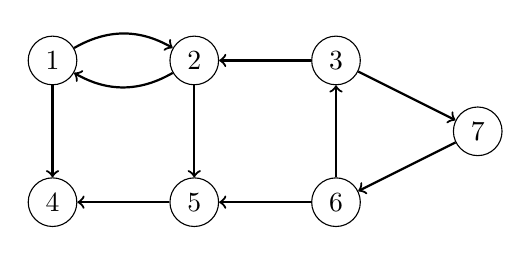
\begin{tikzpicture}[scale=0.9,label distance=-2mm]
\node[draw, circle] (1) at (-1,1) {$7$};
\node[draw, circle] (2) at (-3,2) {$3$};
\node[draw, circle] (4) at (-5,2) {$2$};
\node[draw, circle] (6) at (-7,2) {$1$};
\node[draw, circle] (3) at (-3,0) {$6$};
\node[draw, circle] (5) at (-5,0) {$5$};
\node[draw, circle] (7) at (-7,0) {$4$};

\path[draw,thick,->] (2) -- (1);
\path[draw,thick,->] (1) -- (3);
\path[draw,thick,->] (3) -- (2);
\path[draw,thick,->] (2) -- (4);
\path[draw,thick,->] (3) -- (5);
\path[draw,thick,->] (4) edge [bend left] (6);
\path[draw,thick,->] (6) edge [bend left] (4);
\path[draw,thick,->] (4) -- (5);
\path[draw,thick,->] (5) -- (7);
\path[draw,thick,->] (6) -- (7);
\end{tikzpicture}
\end{center}
берік байланысты компоненттері келесідей:
% the strongly connected components are as follows:
\begin{center}
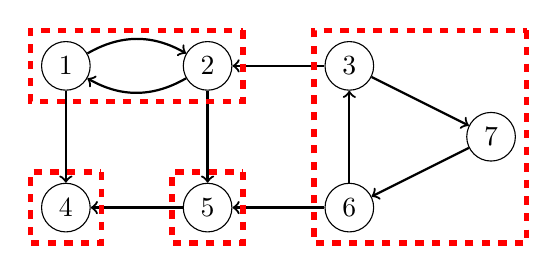
\begin{tikzpicture}[scale=0.9]
\node[draw, circle] (1) at (-1,1) {$7$};
\node[draw, circle] (2) at (-3,2) {$3$};
\node[draw, circle] (4) at (-5,2) {$2$};
\node[draw, circle] (6) at (-7,2) {$1$};
\node[draw, circle] (3) at (-3,0) {$6$};
\node[draw, circle] (5) at (-5,0) {$5$};
\node[draw, circle] (7) at (-7,0) {$4$};

\path[draw,thick,->] (2) -- (1);
\path[draw,thick,->] (1) -- (3);
\path[draw,thick,->] (3) -- (2);
\path[draw,thick,->] (2) -- (4);
\path[draw,thick,->] (3) -- (5);
\path[draw,thick,->] (4) edge [bend left] (6);
\path[draw,thick,->] (6) edge [bend left] (4);
\path[draw,thick,->] (4) -- (5);
\path[draw,thick,->] (5) -- (7);
\path[draw,thick,->] (6) -- (7);

\draw [red,thick,dashed,line width=2pt] (-0.5,2.5) rectangle (-3.5,-0.5);
\draw [red,thick,dashed,line width=2pt] (-4.5,2.5) rectangle (-7.5,1.5);
\draw [red,thick,dashed,line width=2pt] (-4.5,0.5) rectangle (-5.5,-0.5);
\draw [red,thick,dashed,line width=2pt] (-6.5,0.5) rectangle (-7.5,-0.5);
\end{tikzpicture}
\end{center}

Сәйкес компоненттер графы келесідей:
% The corresponding component graph is as follows:
\begin{center}
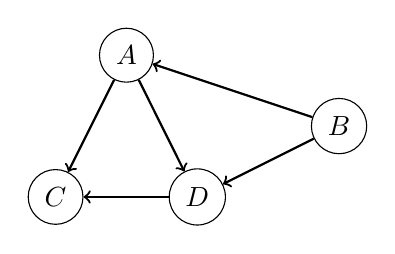
\begin{tikzpicture}[scale=0.9]
\node[draw, circle] (1) at (-3,1) {$B$};
\node[draw, circle] (2) at (-6,2) {$A$};
\node[draw, circle] (3) at (-5,0) {$D$};
\node[draw, circle] (4) at (-7,0) {$C$};

\path[draw,thick,->] (1) -- (2);
\path[draw,thick,->] (1) -- (3);
\path[draw,thick,->] (2) -- (3);
\path[draw,thick,->] (2) -- (4);
\path[draw,thick,->] (3) -- (4);
\end{tikzpicture}
\end{center}
Компоненттер: $A=\{1,2\}$,
$B=\{3,6,7\}$, $C=\{4\}$ және $D=\{5\}$.

Компоненттерден тұратын граф ациклды, бағытталған болады.
Сондықтан бұл графпен жұмыс істеу оңайырақ. Граф цикл қамтымағандықтан
әрқашан да графты топологиялық сұрыптауға немесе 16-тарауда
талқыланған динамикалық бағдарламалау әдістерін қолдануға болады.
% A component graph is an acyclic, directed graph,
% so it is easier to process than the original graph.
% Since the graph does not contain cycles,
% we can always construct a topological sort and
% use dynamic programming techniques like those
% presented in Chapter 16.

\section{Косараджу алгоритмі}

\index{Косараджу алгоритмі}

\key{Косараджу алгоритмі}\footnote{Бұл сілтемеге \cite{aho83} бағынсақ,
С.Р.Косараджу бұл алгоритмді 1978 жылы ойлап тапты, бірақ оны жарияламады. 1981 жылы дәл сол алгоритмді М.Шәрир қайта ашып, жариялады \cite{sha81}.} -- бағытталған графтың берік байланысты компоненттерін 
табудың тиімді әдісі. Алгоритм  тереңдігі бойынша екі
ізденісті қолданады. Біріншісі арқылы графтың құрылымына сәйкес төбелердің
тізімін  құраса, екіншісі арқылы берік байланысты компоненттерді құрайды.
% is an efficient
% method for finding the strongly connected components
% of a directed graph.
% The algorithm performs two depth-first searches:
% the first search constructs a list of nodes
% according to the structure of the graph,
% and the second search forms the strongly connected components.

\subsubsection{1-ізденіс}

Косараджу алгоритмінің бірінші бөлімінде төбелердің тізімін тереңдігі бойынша ізденістің 
жүру ретімен құрайды.
Алгоритм төбелерді біртіндеп өтіп, қандай да бір төбе әлі өңделмеген болса, 
сол төбеден тереңдігі бойынша ізденісті бастайды.
Графтың әр төбесі тізімге өңделгеннен кейін қосылады.
% The first phase of Kosaraju's algorithm constructs
% a list of nodes in the order in which a
% depth-first search processes them.
% The algorithm goes through the nodes,
% and begins a depth-first search at each 
% unprocessed node.
% Each node will be added to the list
% after it has been processed.

Мысалдағы граф төбелерін осы ретпен өңдейді:
% In the example graph, the nodes are processed
% in the following order:
\begin{center}
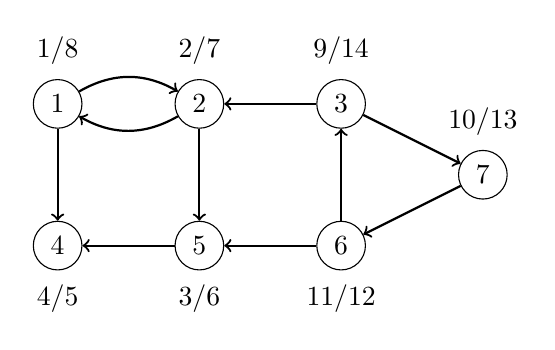
\begin{tikzpicture}[scale=0.9,label distance=-2mm]
\node[draw, circle] (1) at (-1,1) {$7$};
\node[draw, circle] (2) at (-3,2) {$3$};
\node[draw, circle] (4) at (-5,2) {$2$};
\node[draw, circle] (6) at (-7,2) {$1$};
\node[draw, circle] (3) at (-3,0) {$6$};
\node[draw, circle] (5) at (-5,0) {$5$};
\node[draw, circle] (7) at (-7,0) {$4$};

\node at (-7,2.75) {$1/8$};
\node at (-5,2.75) {$2/7$};
\node at (-3,2.75) {$9/14$};
\node at (-7,-0.75) {$4/5$};
\node at (-5,-0.75) {$3/6$};
\node at (-3,-0.75) {$11/12$};
\node at (-1,1.75) {$10/13$};

\path[draw,thick,->] (2) -- (1);
\path[draw,thick,->] (1) -- (3);
\path[draw,thick,->] (3) -- (2);
\path[draw,thick,->] (2) -- (4);
\path[draw,thick,->] (3) -- (5);
\path[draw,thick,->] (4) edge [bend left] (6);
\path[draw,thick,->] (6) edge [bend left] (4);
\path[draw,thick,->] (4) -- (5);
\path[draw,thick,->] (5) -- (7);
\path[draw,thick,->] (6) -- (7);
\end{tikzpicture}
\end{center}

Бұл жерде $x/y$ белгісі төбені өңдеу $x$ уақытында 
басталып, $y$ уақытында аяқталғанын білдіреді.
Сәйкесінше, тізім келесідей болмақ:

% The notation $x/y$ means that
% processing the node started
% at time $x$ and finished at time $y$.
% Thus, the corresponding list is as follows:

\begin{tabular}{ll}
\\
төбе & өңдеу уақыты \\
\hline
4 & 5 \\
5 & 6 \\
2 & 7 \\
1 & 8 \\
6 & 12 \\
7 & 13 \\
3 & 14 \\
\\
\end{tabular}
% 
% In the second phase of the algorithm,
% the nodes will be processed
% in reverse order: $[3,7,6,1,2,5,4]$.

\subsubsection{2-ізденіс}

Косараджу алгоритмінің екінші бөлімінде графтың берік байланысты
компоненттері құрылады.
Алдымен алгоритм графтағы әр қырдың бағытын ауыстырады, яғни қыр бұрын
$a$-төбесінен $b$-төбесіне бағытталса, енді $b$-төбесінен $a$-төбесіне қарай 
бағытталады. 
Бұл екінші іздеу кезінде  
берік байланысты компоненттерді әрқашан 
табатындығымызға толықтай кепілдік береді.
% The second phase of the algorithm
% forms the strongly connected components
% of the graph.
% First, the algorithm reverses every
% edge in the graph.
% This guarantees that during the second search,
% we will always find strongly connected
% components that do not have extra nodes.

Мысалда қырларының бағытын ауыстырғаннан кейінгі
граф берілген:
% After reversing the edges,
% the example graph is as follows:
\begin{center}
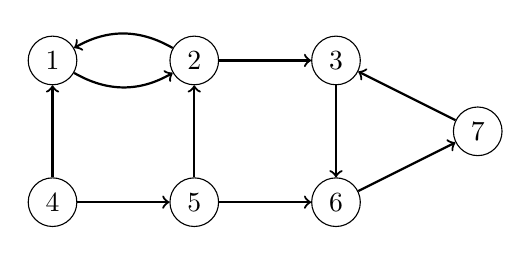
\begin{tikzpicture}[scale=0.9,label distance=-2mm]
\node[draw, circle] (1) at (-1,1) {$7$};
\node[draw, circle] (2) at (-3,2) {$3$};
\node[draw, circle] (4) at (-5,2) {$2$};
\node[draw, circle] (6) at (-7,2) {$1$};
\node[draw, circle] (3) at (-3,0) {$6$};
\node[draw, circle] (5) at (-5,0) {$5$};
\node[draw, circle] (7) at (-7,0) {$4$};

\path[draw,thick,<-] (2) -- (1);
\path[draw,thick,<-] (1) -- (3);
\path[draw,thick,<-] (3) -- (2);
\path[draw,thick,<-] (2) -- (4);
\path[draw,thick,<-] (3) -- (5);
\path[draw,thick,<-] (4) edge [bend left] (6);
\path[draw,thick,<-] (6) edge [bend left] (4);
\path[draw,thick,<-] (4) -- (5);
\path[draw,thick,<-] (5) -- (7);
\path[draw,thick,<-] (6) -- (7);
\end{tikzpicture}
\end{center}

Содан кейін, алгоритм бірінші бөлімде құрылған төбелердің тізімін
\emph{кері ретпен} өтеді.
Егер төбе компонентке жатпаса, алгоритм жаңа компонент құрып, тереңдігі бойынша ізденісті бастайды. Бұл ізденісте өтетін барлық төбелерді қазіргі құрылып жатқан компонентке қосады.
% After this, the algorithm goes through
% the list of nodes created by the first search,
% in \emph{reverse} order.
% If a node does not belong to a component,
% the algorithm creates a new component
% and starts a depth-first search
% that adds all new nodes found during the search
% to the new component.

Мысалдағы графтың бірінші компоненті 3-төбеден басталады:
% In the example graph, the first component
% begins at node 3:

\begin{center}
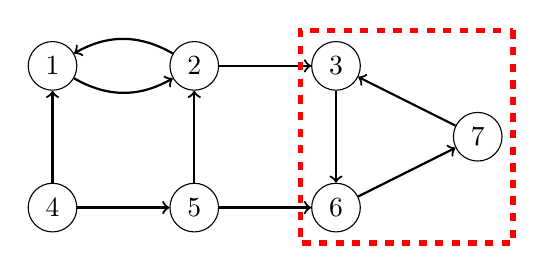
\begin{tikzpicture}[scale=0.9,label distance=-2mm]
\node[draw, circle] (1) at (-1,1) {$7$};
\node[draw, circle] (2) at (-3,2) {$3$};
\node[draw, circle] (4) at (-5,2) {$2$};
\node[draw, circle] (6) at (-7,2) {$1$};
\node[draw, circle] (3) at (-3,0) {$6$};
\node[draw, circle] (5) at (-5,0) {$5$};
\node[draw, circle] (7) at (-7,0) {$4$};

\path[draw,thick,<-] (2) -- (1);
\path[draw,thick,<-] (1) -- (3);
\path[draw,thick,<-] (3) -- (2);
\path[draw,thick,<-] (2) -- (4);
\path[draw,thick,<-] (3) -- (5);
\path[draw,thick,<-] (4) edge [bend left] (6);
\path[draw,thick,<-] (6) edge [bend left] (4);
\path[draw,thick,<-] (4) -- (5);
\path[draw,thick,<-] (5) -- (7);
\path[draw,thick,<-] (6) -- (7);

\draw [red,thick,dashed,line width=2pt] (-0.5,2.5) rectangle (-3.5,-0.5);
\end{tikzpicture}
\end{center}

Барлық қырлардың бағытын ауыстырғандықтан
компонент графтың басқа бөліктеріне ''ағып кетпейді''.
% Note that since all edges are reversed,
% the component does not ''leak'' to other parts in the graph.

\begin{samepage}
Тізімдегі келесі төбелерге 6 және 7-төбелер жатады. Бірақ олар бұрыннан
компоненттің құрамында болғандықтан, келесі компонент 1-төбеден басталады:
% The next nodes in the list are nodes 7 and 6,
% but they already belong to a component,
% so the next new component begins at node 1:

\begin{center}
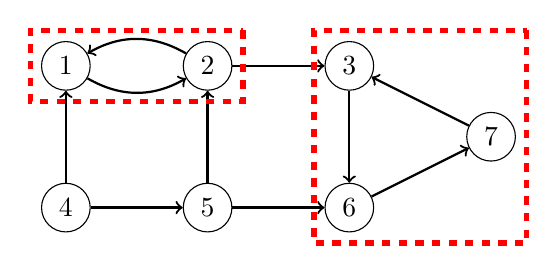
\begin{tikzpicture}[scale=0.9,label distance=-2mm]
\node[draw, circle] (1) at (-1,1) {$7$};
\node[draw, circle] (2) at (-3,2) {$3$};
\node[draw, circle] (4) at (-5,2) {$2$};
\node[draw, circle] (6) at (-7,2) {$1$};
\node[draw, circle] (3) at (-3,0) {$6$};
\node[draw, circle] (5) at (-5,0) {$5$};
\node[draw, circle] (7) at (-7,0) {$4$};

\path[draw,thick,<-] (2) -- (1);
\path[draw,thick,<-] (1) -- (3);
\path[draw,thick,<-] (3) -- (2);
\path[draw,thick,<-] (2) -- (4);
\path[draw,thick,<-] (3) -- (5);
\path[draw,thick,<-] (4) edge [bend left] (6);
\path[draw,thick,<-] (6) edge [bend left] (4);
\path[draw,thick,<-] (4) -- (5);
\path[draw,thick,<-] (5) -- (7);
\path[draw,thick,<-] (6) -- (7);

\draw [red,thick,dashed,line width=2pt] (-0.5,2.5) rectangle (-3.5,-0.5);
\draw [red,thick,dashed,line width=2pt] (-4.5,2.5) rectangle (-7.5,1.5);
%\draw [red,thick,dashed,line width=2pt] (-4.5,0.5) rectangle (-5.5,-0.5);
%\draw [red,thick,dashed,line width=2pt] (-6.5,0.5) rectangle (-7.5,-0.5);
\end{tikzpicture}
\end{center}
\end{samepage}

\begin{samepage}
Соңында алгоритм 5 және 4-төбелді өңдейді. Олар соңғы берік байланысты
компонентті құрайды.
% Finally, the algorithm processes nodes 5 and 4
% that create the remaining strongly connected components:

\begin{center}
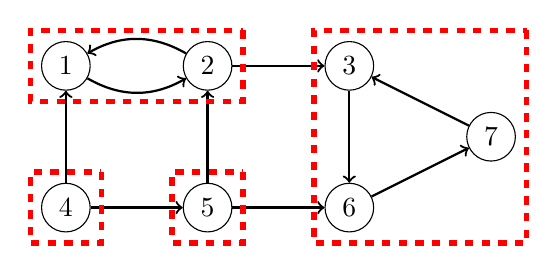
\begin{tikzpicture}[scale=0.9,label distance=-2mm]
\node[draw, circle] (1) at (-1,1) {$7$};
\node[draw, circle] (2) at (-3,2) {$3$};
\node[draw, circle] (4) at (-5,2) {$2$};
\node[draw, circle] (6) at (-7,2) {$1$};
\node[draw, circle] (3) at (-3,0) {$6$};
\node[draw, circle] (5) at (-5,0) {$5$};
\node[draw, circle] (7) at (-7,0) {$4$};

\path[draw,thick,<-] (2) -- (1);
\path[draw,thick,<-] (1) -- (3);
\path[draw,thick,<-] (3) -- (2);
\path[draw,thick,<-] (2) -- (4);
\path[draw,thick,<-] (3) -- (5);
\path[draw,thick,<-] (4) edge [bend left] (6);
\path[draw,thick,<-] (6) edge [bend left] (4);
\path[draw,thick,<-] (4) -- (5);
\path[draw,thick,<-] (5) -- (7);
\path[draw,thick,<-] (6) -- (7);

\draw [red,thick,dashed,line width=2pt] (-0.5,2.5) rectangle (-3.5,-0.5);
\draw [red,thick,dashed,line width=2pt] (-4.5,2.5) rectangle (-7.5,1.5);
\draw [red,thick,dashed,line width=2pt] (-4.5,0.5) rectangle (-5.5,-0.5);
\draw [red,thick,dashed,line width=2pt] (-6.5,0.5) rectangle (-7.5,-0.5);
\end{tikzpicture}
\end{center}
\end{samepage}

Алгоритмнің уақытша күрделілігі -- $O(n+m)$. Себебі алгоритм 
тереңдігі бойынша екі ізденісті қамтиды.
% The time complexity of the algorithm is $O(n+m)$,
% because the algorithm
% performs two depth-first searches.

\section{2SAT есебі}

\index{2SAT есебі}

Берік байланыстылықтың \key{2SAT есебіне} де қатысы бар\footnote{Мұнда ұсынылған алгоритм осы жерде таныстырылған болатын \cite{asp79}.
Сондай-ақ қайта іздеу   (backtracking) алгоритміне негізделген тағы бір танымал сызықтық уақыттағы күрделі алгоритм бар \cite{eve75}.}.
% Strong connectivity is also linked with the
% \key{2SAT problem}\footnote{The algorithm presented here was
% introduced in \cite{asp79}.
% There is also another well-known linear-time algorithm \cite{eve75}
% that is based on backtracking.}.
Төмендегі есепте бізге логикалық формула беріледі:
% In this problem, we are given a logical formula
\[
(a_1 \lor b_1) \land (a_2 \lor b_2) \land \cdots \land (a_m \lor b_m),
\]
мұндағы $a_i$ және $b_i$ екеуі де логикалық айнымалы
($x_1,x_2,\ldots,x_n$)
немесе логикалық айнымалының терісі
($\lnot x_1, \lnot x_2, \ldots, \lnot x_n$).
''$\land$'' және ''$\lor$'' символдары ''конъюнкция'' (биттік және) және ''дизъюнкция''
(биттік немесе) логикалық операторларын белгілейді.
Есепте берілген тапсырма -- әр айнымалыға формула
ақиқат(true) болатындай мән беру немесе бұл мүмкін
емес екенін анықтау. 
% Our task is to assign each variable a value
% so that the formula is true, or state
% that this is not possible.

Мысалы, осы формулалар үшін
% For example, the formula
\[
L_1 = (x_2 \lor \lnot x_1) \land
      (\lnot x_1 \lor \lnot x_2) \land
      (x_1 \lor x_3) \land
      (\lnot x_2 \lor \lnot x_3) \land
      (x_1 \lor x_4)
\]
айнымалыларға төмендегідей мәндер берілсе, ақиқат болады :
% is true when the variables are assigned as follows:

\[
\begin{cases}
x_1 = \textrm{false} \\
x_2 = \textrm{false} \\
x_3 = \textrm{true} \\
x_4 = \textrm{true} \\
\end{cases}
\]

Дегенмен мына формулада
% However, the formula
\[
L_2 = (x_1 \lor x_2) \land
      (x_1 \lor \lnot x_2) \land
      (\lnot x_1 \lor x_3) \land
      (\lnot x_1 \lor \lnot x_3)
\]
айнымалыларға қандай мән берсе де жалған болады.
Мұның себебі $x_1$ мәнін қарама-қайшылықтарсыз
таңдай алмауымызда жатыр. Егер $x_1$ жалған болса, $x_2$ және $\lnot x_2$ 
де ақиқат болуы қажет еді, бірақ ол мүмкін емес. Сонымен қатар, егер $x_1$ ақиқат
болса $x_3$ және $\lnot x_3$ те ақиқат болуы қажет еді, бірақ бұл да мүмкін
емес.
% The reason for this is that we cannot
% choose a value for $x_1$
% without creating a contradiction.
% If $x_1$ is false, both $x_2$ and $\lnot x_2$
% should be true which is impossible,
% and if $x_1$ is true, both $x_3$ and $\lnot x_3$
% should be true which is also impossible.

2SAT есебін граф сияқты қарастыруға болады. Бұл графта
төбелер $x_i$ және теріс $\lnot x_i$ айнымалыларына
сәйкес, ал қырлар  айнымалылар арасындағы арақатынасты белгілейді.
Әр $(a_i \lor b_i)$ жұбы екі қыр жасайды: 
$\lnot a_i \to b_i$ және $\lnot b_i \to a_i$.
Бұл $a_i$ орындалмаса, $b_i$ орындалуы қажет немесе
керісінше $b_i$ орындалмаса, $a_i$ орындалуы қажет деген арақатынасты білдіреді. 
% Бұл -- $a_i$ болмаса, $b_i$ болуы керек екендігін көрсету
% және керісінше жұмыс істейді.
% The 2SAT problem can be represented as a graph
% whose nodes correspond to
% variables $x_i$  and negations $\lnot x_i$,
% and edges determine the connections
% between the variables.
% Each pair $(a_i \lor b_i)$ generates two edges:
% $\lnot a_i \to b_i$ and $\lnot b_i \to a_i$.
% This means that if $a_i$ does not hold,
% $b_i$ must hold, and vice versa.

$L_1$ формуласының графы:
% The graph for the formula $L_1$ is:
\\
\begin{center}
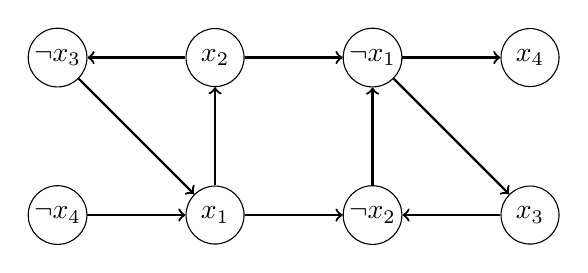
\begin{tikzpicture}[scale=1.0,minimum size=2pt]
\node[draw, circle, inner sep=1.3pt] (1) at (1,2) {$\lnot x_3$};
\node[draw, circle] (2) at (3,2) {$x_2$};
\node[draw, circle, inner sep=1.3pt] (3) at (1,0) {$\lnot x_4$};
\node[draw, circle] (4) at (3,0) {$x_1$};
\node[draw, circle, inner sep=1.3pt] (5) at (5,2) {$\lnot x_1$};
\node[draw, circle] (6) at (7,2) {$x_4$};
\node[draw, circle, inner sep=1.3pt] (7) at (5,0) {$\lnot x_2$};
\node[draw, circle] (8) at (7,0) {$x_3$};
 
\path[draw,thick,->] (1) -- (4);
\path[draw,thick,->] (4) -- (2);
\path[draw,thick,->] (2) -- (1);
\path[draw,thick,->] (3) -- (4);
\path[draw,thick,->] (2) -- (5);
\path[draw,thick,->] (4) -- (7);
\path[draw,thick,->] (5) -- (6);
\path[draw,thick,->] (5) -- (8);
\path[draw,thick,->] (8) -- (7);
\path[draw,thick,->] (7) -- (5);
\end{tikzpicture}
\end{center}
Ал $L_2$ формуласының графы:
% And the graph for the formula $L_2$ is:
\\
\begin{center}
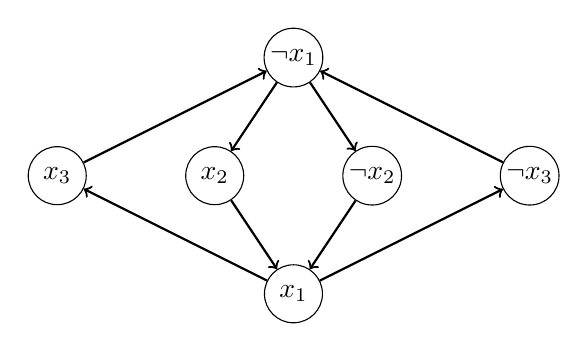
\begin{tikzpicture}[scale=1.0,minimum size=2pt]
\node[draw, circle] (1) at (1,2) {$x_3$};
\node[draw, circle] (2) at (3,2) {$x_2$};
\node[draw, circle, inner sep=1.3pt] (3) at (5,2) {$\lnot x_2$};
\node[draw, circle, inner sep=1.3pt] (4) at (7,2) {$\lnot x_3$};
\node[draw, circle, inner sep=1.3pt] (5) at (4,3.5) {$\lnot x_1$};
\node[draw, circle] (6) at (4,0.5) {$x_1$};

\path[draw,thick,->] (1) -- (5);
\path[draw,thick,->] (4) -- (5);
\path[draw,thick,->] (6) -- (1);
\path[draw,thick,->] (6) -- (4);
\path[draw,thick,->] (5) -- (2);
\path[draw,thick,->] (5) -- (3);
\path[draw,thick,->] (2) -- (6);
\path[draw,thick,->] (3) -- (6);
\end{tikzpicture}
\end{center}

Графтың құрылымы айнымалыларға формуланы ақиқат ететіндей
мән беруге болатынын немесе болмайтындығын көрсетеді.
Егер әр $x_i$ және $\lnot x_i$ 
төбелері бөлек берік байланысты
компоненттерге жатса ғана, формуланы ақиқат деуге болады.
Егер бір берік байланыстылық компонентінде $x_i$ және $\lnot x_i$ қамтылса, граф $x_i$-төбеден $\lnot x_i$-төбеге 
және $\lnot x_i$-төбеден $x_i$-төбеге апаратын жолдардан тұрады. Сондықтан олар бір уақытта тең ақиқат
болулары қажет, бірақ бұл мүмкін емес.
% The structure of the graph tells us whether
% it is possible to assign the values
% of the variables so
% that the formula is true.
% It turns out that this can be done
% exactly when there are no nodes
% $x_i$ and $\lnot x_i$ such that
% both nodes belong to the
% same strongly connected component.
% If there are such nodes,
% the graph contains
% a path from $x_i$ to $\lnot x_i$
% and also a path from $\lnot x_i$ to $x_i$,
% so both $x_i$ and $\lnot x_i$ should be true
% which is not possible.

$L_1$ формуласының графында ешқандай $x_i$ және $\lnot x_i$ жұбы бір
берік байналысты компонентке жатпайды. Сондықтан шешімі болады.
Ал $L_2$ формуласының графында барлық төбелер бір берік байланысты
компонентке жатады, сол себепті де шешімі жоқ.

% In the graph of the formula $L_1$
% there are no nodes $x_i$ and $\lnot x_i$
% such that both nodes 
% belong to the same strongly connected component,
% so a solution exists.
% In the graph of the formula $L_2$
% all nodes belong to the same strongly connected component,
% so a solution does not exist.

Егер шешім бар болса, айнымалының мәндерін кері топологиялық сұрыптау ретімен компоненттер графының төбелерін өту арқылы табуға болады. Біз әрбір қадамда өңделмеген компонентке бағытталған қырды қамтымайтын компонентті қарастырамыз. Егер компоненттердегі айнымалыларға мән 
берілмесе, олардың мәндері компоненттегі мәндерге 
сәйкес анықталады, ал егер олардың мәндері әлдеқашан бар болса,
олар өзгеріссіз қалады. Осы процесс әр айнымалыға мән тағайындалғанша жалғасады.
% If a solution exists, the values for the variables
% can be found by going through the nodes of the
% component graph in a reverse topological sort order.
% At each step, we process a component 
% that does not contain edges that lead to an
% unprocessed component.
% If the variables in the component
% have not been assigned values,
% their values will be determined
% according to the values in the component,
% and if they already have values,
% they remain unchanged.
% The process continues until each variable
% has been assigned a value.

$L_1$ формуласының компонентті графы:
% The component graph for the formula $L_1$ is as follows:
\begin{center}
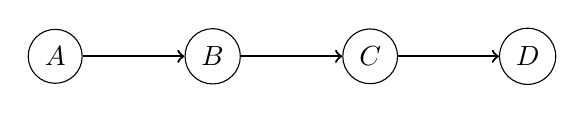
\begin{tikzpicture}[scale=1.0]
\node[draw, circle] (1) at (0,0) {$A$};
\node[draw, circle] (2) at (2,0) {$B$};
\node[draw, circle] (3) at (4,0) {$C$};
\node[draw, circle] (4) at (6,0) {$D$};

\path[draw,thick,->] (1) -- (2);
\path[draw,thick,->] (2) -- (3);
\path[draw,thick,->] (3) -- (4);
\end{tikzpicture}
\end{center}

Бұл жердегі компоненттерге
$A = \{\lnot x_4\}$,
$B = \{x_1, x_2, \lnot x_3\}$,
$C = \{\lnot x_1, \lnot x_2, x_3\}$ және
$D = \{x_4\}$ жатады.
Шешімді құрып жатқанда, алдымен
$D$ компонентін өңдейміз. Сол кезде $x_4$ айнымалысына
ақиқат мәні беріледі. Кейін біз $C$ компонентін
өңдейміз. Бұл жерде $x_1$ және $x_2$ айнымалысы жалған болып,
$x_3$ айнымалысы ақиқат болады. Барлық айнымалыға мән беріледі.
Сондықтан қалған $A$ және $B$ компоненттері айнымалылардың мәндерін өзгертпейді.
% When constructing the solution,
% we first process the component $D$
% where $x_4$ becomes true.
% After this, we process the component $C$
% where $x_1$ and $x_2$ become false
% and $x_3$ becomes true.
% All variables have been assigned values,
% so the remaining components $A$ and $B$
% do not change the variables.

Графтың арнайы
құрылымы болғандықтан бұл әдістің тиімді болатындығын есте сақтағанымыз жөн, себебі егер $x_i$-төбесінен $x_j$-төбесіне және 
$x_j$-төбесінен $\lnot x_j$-төбесіне жол болса, мұндай жағдайда $x_i$ төбесі
ешқашан ақиқат бола алмайды. Себебі мұндай жағдайда
$\lnot x_j$-төбесінен $\lnot x_i$-төбесіне де жол болады. Демек $x_i$ және $x_j$ жалған болады.
% Note that this method works, because the
% graph  has a special structure:
% if there are paths from node $x_i$ to node $x_j$
% and from node $x_j$ to node $\lnot x_j$,
% then node $x_i$ never becomes true.
% The reason for this is that there is also
% a path from node $\lnot x_j$ to node $\lnot x_i$,
% and both $x_i$ and $x_j$ become false.

\index{3SAT есебі}

Бұдан қиынырақ есепке 3SAT есебі жатады. Бұл есепте формуланың
әр бөлімі төмендегідей түрден тұрады: $(a_i \lor b_i \lor c_i)$.
Есеп NP-қиын есептерге жататындықтан, шешуін тиімді табатын алгоритм әлі белгісіз болып тұр.
% A more difficult problem is the \key{3SAT problem},
% where each part of the formula is of the form
% $(a_i \lor b_i \lor c_i)$.
% This problem is NP-hard, so no efficient algorithm
% for solving the problem is known.
